\section{On Scheduling Tasks with Quick Recovery from Failure}
% CM Krishna and Kang G Shin
Proposes a dynamic programming algorithm that ensure that backup or contingency schedules can be embedded in original primary schedule so that hard real time deadlines continues to be met in the face of upto maximum number of processor failure.
\subsection*{Key Idea}
The main aim of this approach is to create a limp mode schedule mechanism, where in spite of failure to few available processor nodes, system is able to meet its real time constraints.
The optimization criterion uses cost function, which corresponds to the feedback delay incurred in the control network. \\
Tasks are run periodically and each instance is known as version. 
Multiple copies of versions are called \textit{clones}. There are two types of clones: primary and ghost. A ghost clone is a backup copy which remains dormant until it is activated to take the place of corresponding primary or another ghost whose processor has failed.
\subsection*{Concepts}
An algorithm \textit{P} is considered consisting of two components: \textit{P1} and \textit{P2}.
P1 finds the optimal allocation of tasks to processor and also optimal schedule by calling P2 which is an optimum scheduler for uniprocessor systems.
\subsection*{Problem Statement}
Develop and algorithm Q, that can be used in conjunction with P1 and P2 to obtain an optimal schedule when enough ghosts are incorporated into the schedule to handle N$_{sus}$ processor failures.\\
Schedules designed are considered to be locally preemptive and globally non-preemptive to reduce interconnect overloads.\\
\begin{minipage}{\linewidth}% to keep image and caption on one page
	\makebox[\linewidth]{%        to center the image
		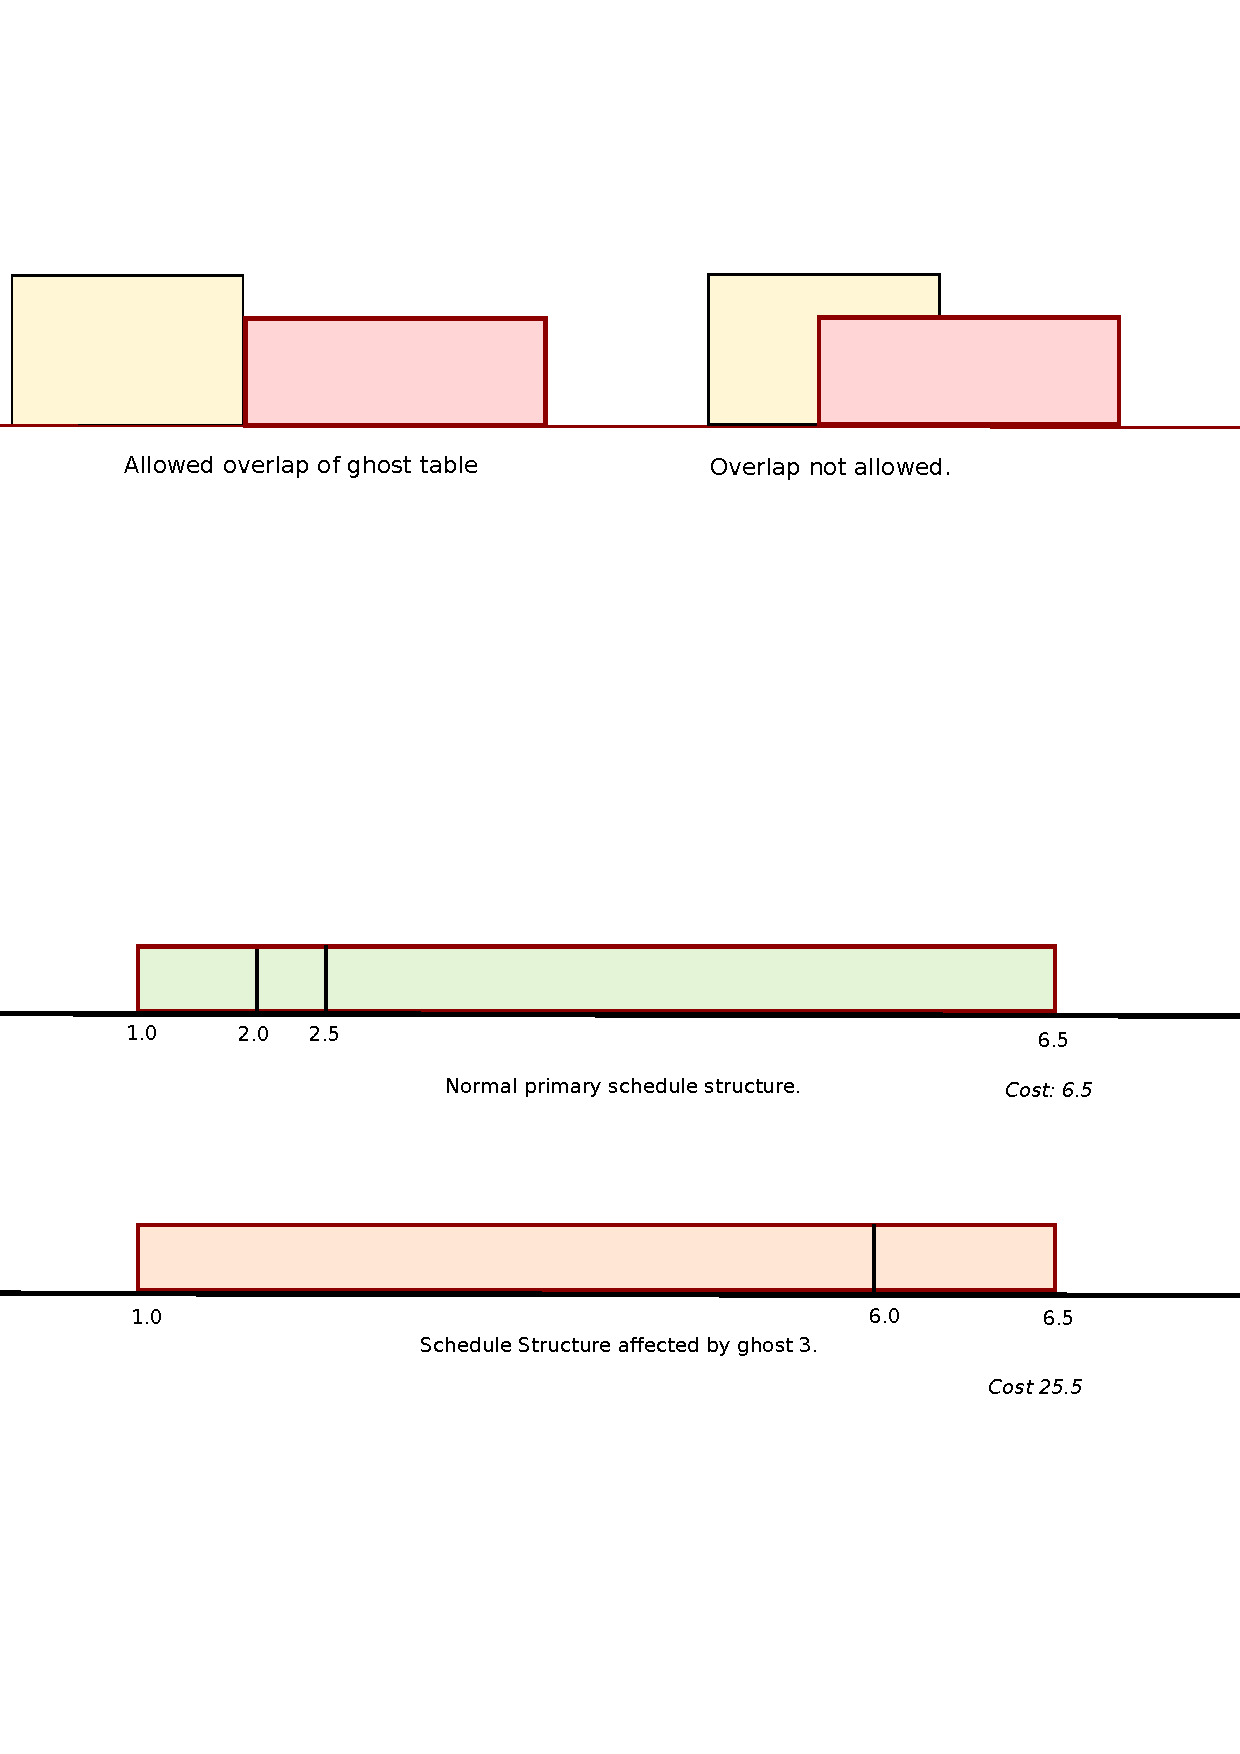
\includegraphics[scale=0.52]{Pictures/paper08_schedule.pdf}}
\end{minipage}
\\
\subsection*{Scheduling mechanism}
Dynamic programming to find the slack holes existing with in the primary schedules. Now do compactness to generate extended holes to schedule ghosts, such that compactness allows the primary tasks to meet there deadlines. In a way similar to the elastic scheduling approach where each task is compacted with restriction being the elasticity coefficient.
\subsection*{conclusion}
A partitioned schedule table driven approach with slack stealing across the cores in case of failure. Its main difference from traditional slack stealing is that, the alternate schedule tables are kept on other processors to be activated in case of failure of the primary schedule. And the activation of the ghost table should not in any way act upon the primary table on the given core.